%!TEX root = ../thesis_a4.tex
% Some new commands for setting up appendices
\newcommand\contrib[1]{\\~{\footnotesize (#1)}}
% 
\newcommand\resource[2]{
	\noindent #1 \par
	\vspace{0.2em}
	{\centering	\url{#2} \par}
	\vspace{0.5em}
	\hrule \par 
	\vspace{0.8em} \par}
%
%
\chapter[Publications by the author][Publications by the author]{Publications by the author}\label{app:mypapers}% by the author

We here provide a list of publications by the author related with the thesis work. For the publications where the role is not that of the first author we  also specify the contributions. Wherever not specified, the contributions are mainly in the formulation of the research problem, building the dataset, writing the code, performing the experiments, analyzing the results and writing the manuscript.

\subsection*{Peer-reviewed journals}
\begin{itemize}[leftmargin=*]
	\item \textbf{Gulati, S.}, Bellur, A., Salamon, J., Ranjani, H., Ishwar, V., Murthy, H. A., \& Serra, X. (2014). Automatic tonic identification in Indian art music: approaches and evaluation. \textit{Journal of New Music Research}, 43(1), 53–71.
	\contrib{Companion webpage: \url{http://compmusic.upf.edu/node/323}}
	\item Koduri, G. K., \textbf{Gulati, S.}, Rao, P., \& Serra, X. (2012). R\={a}ga recognition based on pitch distribution methods. \textit{Journal of New Music Research}, 41(4), 337–350.
	\contrib{Formulating methodology, Writing parts of the code}
	
\end{itemize}
%
\subsection*{Full articles in peer-reviewed conferences}
\begin{itemize}[leftmargin=*]
	\item \textbf{Gulati, S.}, Serr{\`a}, J., Ganguli, K. K., \c{S}ent{\"u}rk, S., \& Serra, X. (2016). Time-delayed melody surfaces for r\={a}ga recognition. In \textit{Proceedings of the 17th International Society for Music Information Retrieval Conference (ISMIR)}, pp. 751–757. New York, USA.
	\contrib{Companion webpage: \url{http://compmusic.upf.edu/node/300}}
	%
	\item Ganguli, K. K., \textbf{Gulati, S.}, Serra, X., \& Rao, P. (2016). Data-driven exploration of melodic structures in Hindustani music. In \textit{Proceedings of the 17th International Society for Music Information Retrieval Conference (ISMIR)}, pp. 605-611. New York, USA.
	\contrib{Formulation of the problem, building dataset, writing the code, writing the manuscript.}
	%
	\item \textbf{Gulati, S.}, Serr{\`a}, J., Ishwar, V., \c{S}ent{\"u}rk, S., \& Serra, X. (2016). Phrase-based r\={a}ga recognition using vector space modeling. In \textit{Proceedings of the 41st IEEE International Conference on Acoustics, Speech and Signal Processing (ICASSP)} , pp. 66–70. Shanghai, China.
	\contrib{Companion webpage: \url{http://compmusic.upf.edu/node/278}}
	%
	\item \textbf{Gulati, S.}, Serr{\`a}, J., Ishwar, V., \& Serra, X. (2016). Discovering r\={a}ga motifs by characterizing communities in networks of melodic patterns. In \textit{Proceedings of the 41st IEEE International Conference on Acoustics, Speech and Signal Processing (ICASSP)}, pp. 286–290. Shanghai, China.
	\contrib{Companion webpage: \url{http://compmusic.upf.edu/node/277}}
	%
	\item \textbf{Gulati, S.}, Serr{\`a}, J., \& Serra, X. (2015). Improving melodic similarity in Indian art music using culture-specific melodic characteristics. In \textit{Proceedings of the 16th International Society for Music Information Retrieval Conference (ISMIR)}, pp. 680–686. M{\'a}laga, Spain.
	\contrib{Companion webpage: \url{http://compmusic.upf.edu/node/269}}
	%
	\item \textbf{Gulati, S.}, Serr{\`a}, J., \& Serra, X. (2015). An evaluation of methodologies for melodic similarity in audio recordings of Indian art music. In \textit{Proceedings of the 40th IEEE International Conference on Acoustics, Speech and Signal Processing (ICASSP)}, pp. 678–682. Brisbane, Australia.
	\contrib{Companion webpage: \url{http://compmusic.upf.edu/node/242}}
	%
	\item \textbf{Gulati, S.},  Serr{\`a}, J., Ishwar, V., \& Serra, X. (2014). Mining melodic patterns in large audio collections of Indian art music. In \textit{Proceedings of the International Conference on Signal Image Technology \& Internet Based Systems (SITIS-MIRA)}, pp. 264–271. Marrakesh, Morocco.
	\contrib{Companion webpage: \url{http://compmusic.upf.edu/node/210}}
	%
	\item \textbf{Gulati, S.}, Serr{\`a}, J., Ganguli, K. K., \& Serra, X. (2014). Landmark detection in Hindustani music melodies. In \textit{Proceedings of the International Computer Music Conference / Sound and Music Computing Conference (ICMC-SMC)}. Athens, Greece. 
	\contrib{Companion webpage: \url{http://compmusic.upf.edu/node/324}}
	%
	\item Srinivasamurthy, A., Koduri, G. K., \textbf{Gulati, S.}, Ishwar, V., \& Serra, X. (2014). Corpora for Music Information Research in Indian Art Music. In \textit{Proceedings of Joint International Computer Music Conference/Sound and Music Computing Conference}. Athens, Greece. 
	\contrib{Compilation of research corpora. Companion webpage: \url{http://compmusic.upf.edu/smc-2014-corpora}}
	%
	\item \c{S}ent{\"u}rk, S., \textbf{Gulati, S.}, \& Serra, X. (2014). Towards alignment of score and audio recordings of ottoman-turkish makam music. In \textit{Proceedings of the 4th International Workshop on Folk Music Analysis (FMA)}. Istanbul, Turkey. 
	\contrib{Ask Sertan}
	%
	\item Bogdanov, D., Wack, N., G{\'o}mez, E., \textbf{Gulati, S.}, Herrera, P., Mayor, O., Roma, G., Salamon, J., Zapata, J., \& Serra, X. (2013). Essentia: an audio analysis library for music information retrieval. In \textit{Proceedings of the 14th International Society for Music Information Retrieval Conference (ISMIR)}, pp. 493–498. Curitiba, Brazil.
	\contrib{Implementation of tonic identification in Essentia}
	%
	\item Bogdanov, D., Wack, N., G{\'o}mez, E., \textbf{Gulati, S.}, Herrera, P., Mayor, O., Roma, G., Salamon, J., Zapata, J., \& Serra, X. (2013). ESSENTIA: an open-source library for sound and music analysis. In \textit{Proceedings of the 21st ACM international conference on Multimedia}, pp. 855–858. Barcelona, Spain.
	\contrib{Implementation of tonic identification in Essentia}	
	%	
	\item \c{S}ent{\"u}rk, \textbf{S., Gulati, S.}, \& Serra, X. (2013). Score informed tonic identification for makam music of turkey. In \textit{Proceedings of the 14th International Society for Music Information Retrieval Conference (ISMIR)}, pp. 175–180. Curitiba, Brazil.
	\contrib{Ask Sertan}
	%
	\item Sordo, M., Koduri, G. K., \c{S}ent{\"u}rk, S., \textbf{Gulati, S.}, \& Serra, X. (2012). A musically aware system for browsing and interacting with audio music collections. In \textit{Proceedings of the 2nd CompMusic Workshop}. Istanbul, Turkey.
	\contrib{Compilation of research corpora}
	%
	\item Koduri, G. K., \textbf{Gulati, S.}, \& Rao, P. (2011). A survey of raaga recognition techniques and improvements to the state-of-the-art. In \textit{Proceedings of the Sound and Music Computing Conference (SMC)}. Padova, Italy.
	\contrib{Formulating methodology, Writing parts of the code}
	%	
\end{itemize}
%
\subsection*{Other contributions to conferences}
\begin{itemize}[leftmargin=*]
	\item Late breaking demo
	%
	\item \textbf{Gulati, S.}, Ganguli, K. K., Gupta, S., Srinivasamurthy, A., \& Serra, X. (2015). \gls{ragawise}: A Lightweight Real-time Raga Recognition System for Indian Art Music. In Late-Breaking Demo Session of the 16th International Society for Music Information Retrieval Conference. Malaga, Spain. 
	\contrib{Companion webpage: \url{http://compmusic.upf.edu/node/281}}
	%
	\item Caro, R., Srinivasamurthy, A., \textbf{Gulati, S.}, \& Serra, X. (2014). Jingju music: Concepts and Computational Tools for its Analysis. A Tutorial in the 15th International Society for Music Information Retrieval Conference, Taipei, Taiwan. 
	\contrib{Presented the melody part of the tutorial, focused on melodic analysis tools for {jingju} music. Companion webpage:  \url{http://compmusic.upf.edu/jingju-tutorial}}
	
\end{itemize}
%
%Other publications
%
%Other non peer reviewed 
%hacks, reports, 
\chapter{Resources}\label{app:resources}
% <<Whatever could not make it to the main text>>
%This appendix is a compendium of links to resources and additional material related to the work presented in the thesis. An up-to-date set of links is also listed and maintained on the companion webpage \url{http://compmusic.upf.edu/phd-thesis-ajay} or its mirror at \url{www.ajaysrinivasamurthy.in/phd-thesis} . Latest updates on the CompMusic project can be obtained from \url{http://compmusic.upf.edu/}. 
%
%Some of the results not reported in the dissertation and audio examples showcasing the results are presented on the companion webpage. The companion webpage will also be updated with any additional resources and material that will be built in the future. 
%%
%\section*{Music concepts and audio examples}
%\resource{A resource page for Carnatic  pl{tala}, with additional explanation of the structure of many different  pl{tala} and audio examples of music pieces in popular Carnatic  pl{tala}}{http://compmusic.upf.edu/examples-taala-carnatic}
%%
%\resource{A resource page for Hindustani  pl{taal}, with additional explanation of the structure of many different  pl{taal} and audio examples of music pieces in popular Hindustani  pl{taal}}{http://compmusic.upf.edu/examples-taal-hindustani}
%%
%\resource{Audio examples for the different percussion instruments used in Beijing opera}{http://compmusic.upf.edu/examples-percussion-bo}
%%
%\resource{A resource page for percussion patterns in Beijing opera, including scores and audio examples of popular percussion patterns}{http://compmusic.upf.edu/bo-perc-patterns}
%%
%\resource{A resource page for \textit{usul}, the cyclic rhythmic framework in Turkish makam music, with audio examples and scores}{http://compmusic.upf.edu/examples-usul-mmt}
%%
%\section*{Corpora and datasets}
%Access to the corpora and datasets will be through the Dunya API that provides access to audio recordings, metadata and features. Standalone archives of datasets are also distributed in some cases outside of the Dunya API. All the research corpora and datasets related to the thesis are additionally listed at the links below. 
%\begin{description}
%	\item[Research corpora] - \url{http://compmusic.upf.edu/corpora}
%	\item[Test datasets] - \url{http://compmusic.upf.edu/datasets}
%\end{description}
%% 
%\resource{The Dunya Carnatic collection on MusicBrainz that forms the CompMusic Carnatic music research corpus}{http://musicbrainz.org/collection/f96e7215-b2bd-4962-b8c9-2b40c17a1ec6}
%% 
%\resource{The Dunya Hindustani collection on MusicBrainz that forms the CompMusic Hindustani music research corpus}{http://musicbrainz.org/collection/213347a9-e786-4297-8551-d61788c85c80}
%% 
%\resource{The  {CMDo} on MusicBrainz with openly accessible music}{http://musicbrainz.org/collection/a163c8f2-b75f-4655-86be-1504ea2944c2}
%%
%\resource{The  {HMDo} on MusicBrainz with openly accessible music}{http://musicbrainz.org/collection/6adc54c6-6605-4e57-8230-b85f1de5be2b}
%%
%\resource{The  {CMDf} containing rhythm annotated pieces of Carnatic music, from which a subset  {CMDs} dataset is also available}{http://compmusic.upf.edu/carnatic-rhythm-dataset}
%%
%\resource{The  {HMDf} containing rhythm annotated pieces of Hindustani music, from which two subsets  {HMDs} and  {HMDl} datasets are also available}{http://compmusic.upf.edu/hindustani-rhythm-dataset}
%%
%\resource{The  {AMSD} containing audio examples of individual strokes of the mridangam in various tonics}{http://compmusic.upf.edu/mridangam-stroke-dataset}
%%
%\resource{The  {UMSD} containing a transcribed collection of two  {tani avartana} played by the renowned mridangam maestro Padmavibhushan Umayalpuram K. Sivaraman}{http://compmusic.upf.edu/mridangam-tani-dataset}
%%
%\resource{The  {TSD} containing a transcribed collection of tabla solo audio recordings spanning compositions from six different  pl{gharana} of  {tabla}, compiled from the album \textit{Shades of Tabla} by Pandit Arvind Mulgaonkar}{http://compmusic.upf.edu/tabla-solo-dataset}
%% 
%\resource{The  {BOPI} containing isolated strokes spanning the four percussion instrument classes used in Beijing opera}{http://compmusic.upf.edu/bo-perc-dataset}
%%
%\pagebreak % Extra careful here!!!
%\resource{The  {BOPP} containing a collection of audio percussion patterns covering five pattern classes in Beijing opera}{http://compmusic.upf.edu/bopp-dataset}
%% 
%\section*{Results}
%An extended set of results, along with a few audio examples analyzed with the models and algorithms presented in the dissertation are available on the companion page.
%\begin{description}[style=nextline]
%	\item[Audio examples] {\small \url{http://compmusic.upf.edu/phd-thesis-ajay\#examples}}
%	\item[Extended results] {\small \url{http://compmusic.upf.edu/phd-thesis-ajay\#results}}
%\end{description}
%% 
%\section*{Tools and code}
%The links to tools and code related to the thesis are listed. Up-to-date links to code (including future releases) will be available on: \url{http://compmusic.upf.edu/phd-thesis-ajay\#code}
%\begin{description}[style=nextline,font=\normalfont]
%	\item[Essentia audio analysis library] \url{http://essentia.upf.edu/}
%	\item[Dunya API] \url{https://github.com/MTG/pycompmusic}
%	\item[Dunya front end] \url{http://dunya.compmusic.upf.edu/}
%	\item[Dunya server and back end] \url{https://github.com/MTG/dunya}
%	\item[A MATLAB package for meter analysis (Florian Krebs)] \url{https://github.com/flokadillo/bayesbeat}
%	\item[A MATLAB package for beat tracking evaluation (Matthew Davies)] {\footnotesize \url{https://code.soundsoftware.ac.uk/projects/beat-evaluation/}}
%	%\item[An implementation of  {RLCS} by Swapnil Gupta]{https://github.com/swapnilgt/tablaPercPatternsISMIR}
%	\item[Rhythm analysis tools for jingju, from the tutorial in ISMIR 2014] \url{http://compmusic.upf.edu/jingju-tutorial}
%	\item[Sawaal-Jawaab Code and Demo] \url{http://compmusic.upf.edu/ismir-15-hacks}
%	\item[Sonic Visualizer, for visualization and annotation of audio] \url{http://www.sonicvisualiser.org/}
%	\item[BeatStation, an interface to record beat tapping] \url{https://github.com/ajaysmurthy/beatStation}
%\end{description}
%% Discuss specific datasets and code, with links, explain the dataset organization, access. 
%%one idea: identify recorded cycles which are very close to the depicted patterns, and provide them as acoustic documentation on a website and multimedia appendix to the thesis
%

\chapter{Additional Material}\label{app:additional_material}

\begin{figure}[h]
	\begin{center}
		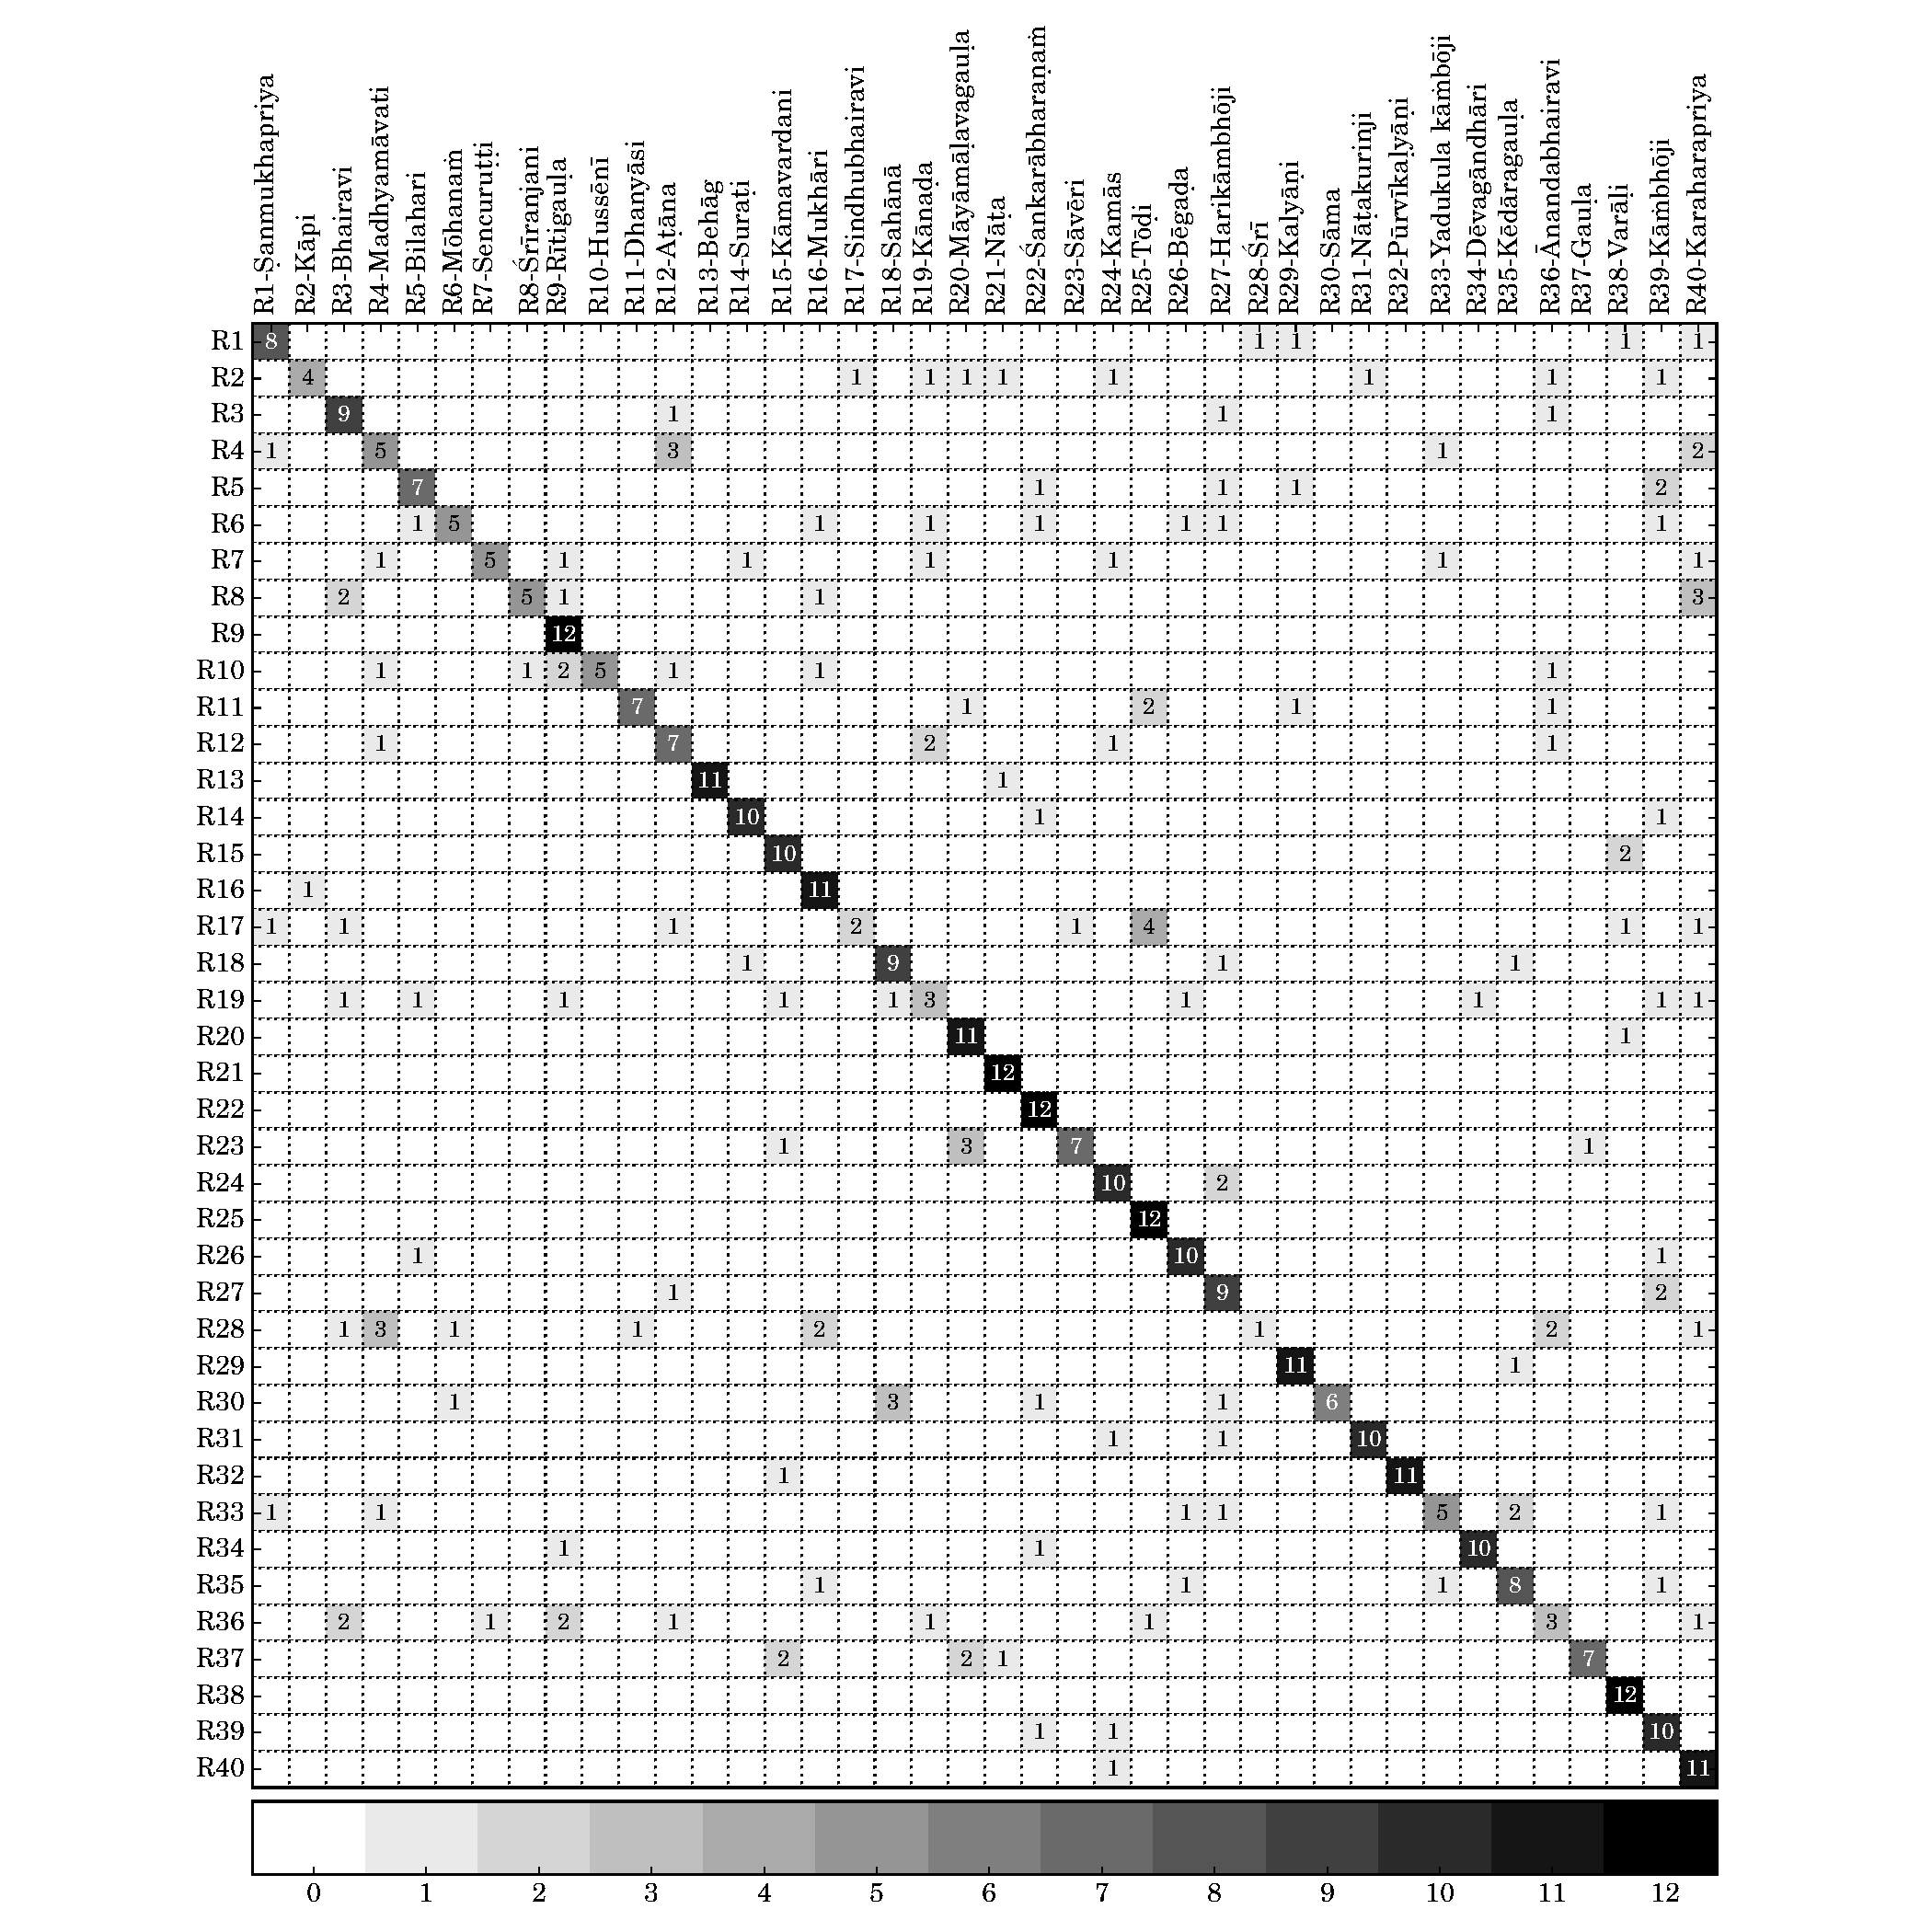
\includegraphics[width=\figSizeNinety]{ch07_ragaRecognition/figures/CM_vsm_cmd_var1.pdf}
	\end{center}
	\caption{Confusion matrix of the \gls{raga} predictions by \acrshort{sotaChordia} on \acrshort{rrds_cmd_big} dataset. The different shades of grey are mapped to different number of audio recordings.}
	\label{fig:confusion_matrix_cmd_chordia}
\end{figure}

\begin{figure}[h]
	\begin{center}
		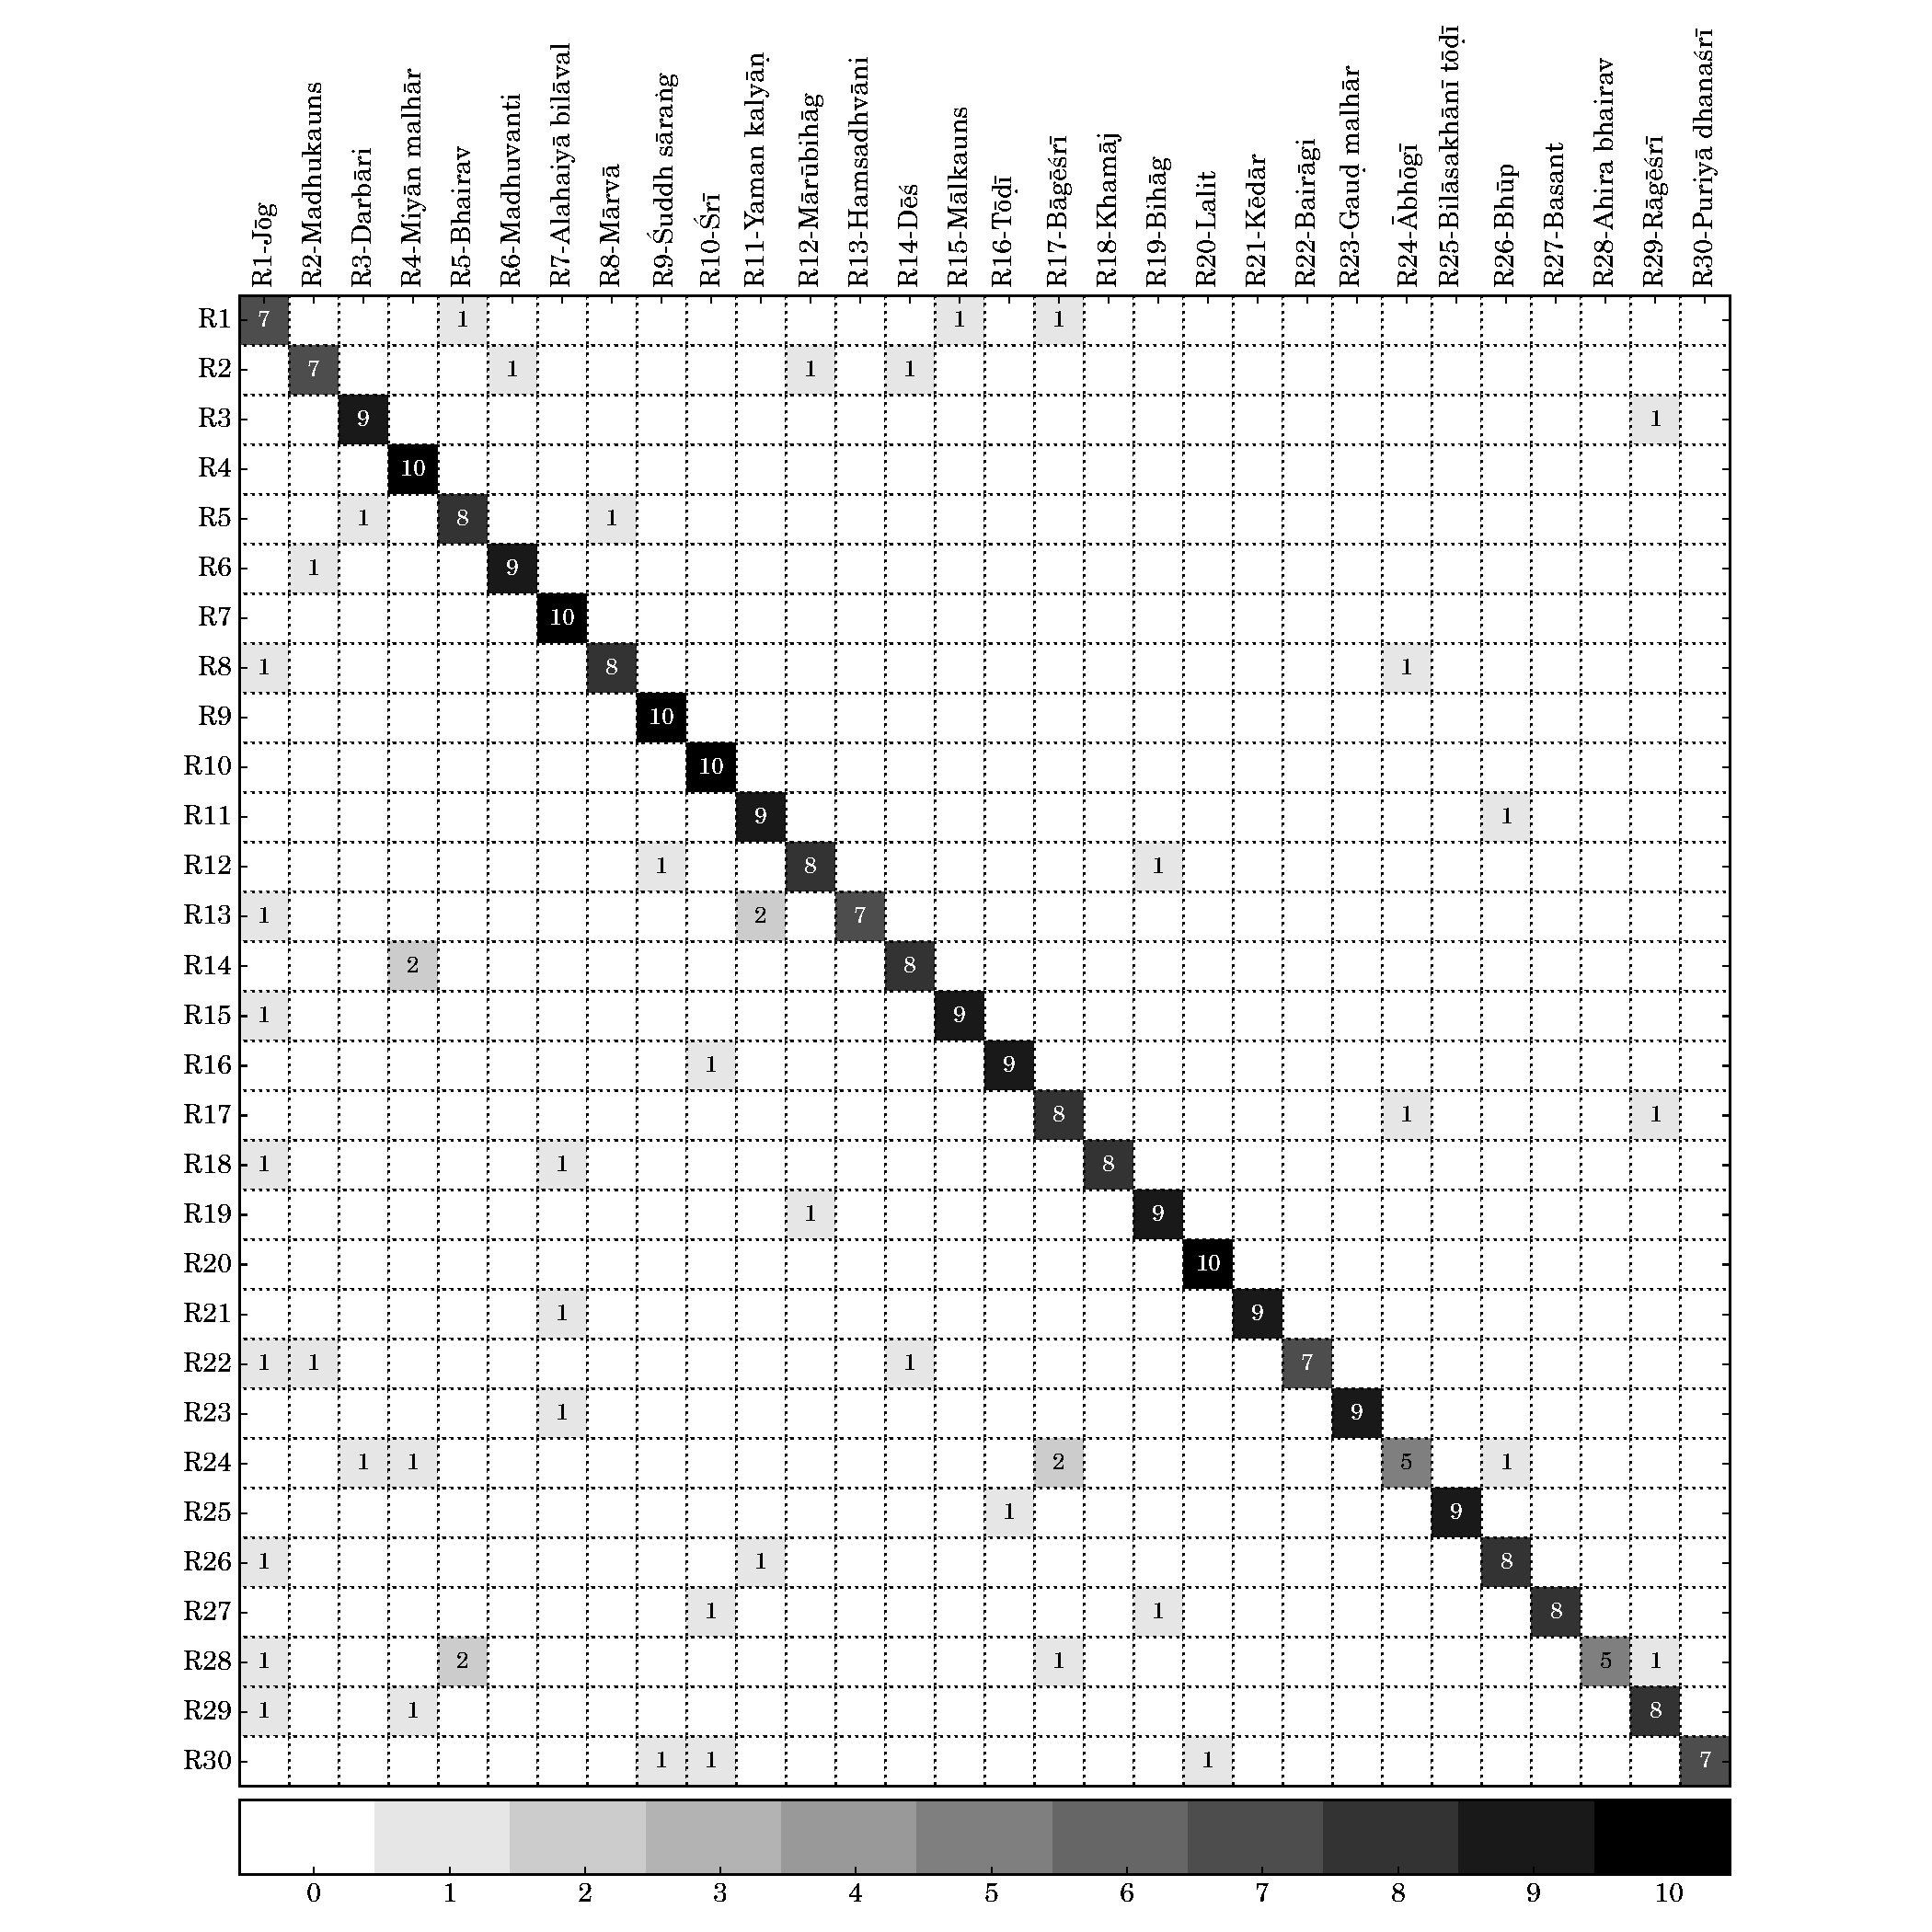
\includegraphics[width=\figSizeNinety]{ch07_ragaRecognition/figures/CM_vsm_hmd_var1.pdf}
	\end{center}
	\caption{Confusion matrix of the \gls{raga} predictions by \acrshort{sotaChordia} on \acrshort{rrds_hmd_big} dataset. The different shades of grey are mapped to different number of audio recordings.}
	\label{fig:confusion_matrix_hmd_chordia}
\end{figure}



\begin{figure}[h]
	\begin{center}
		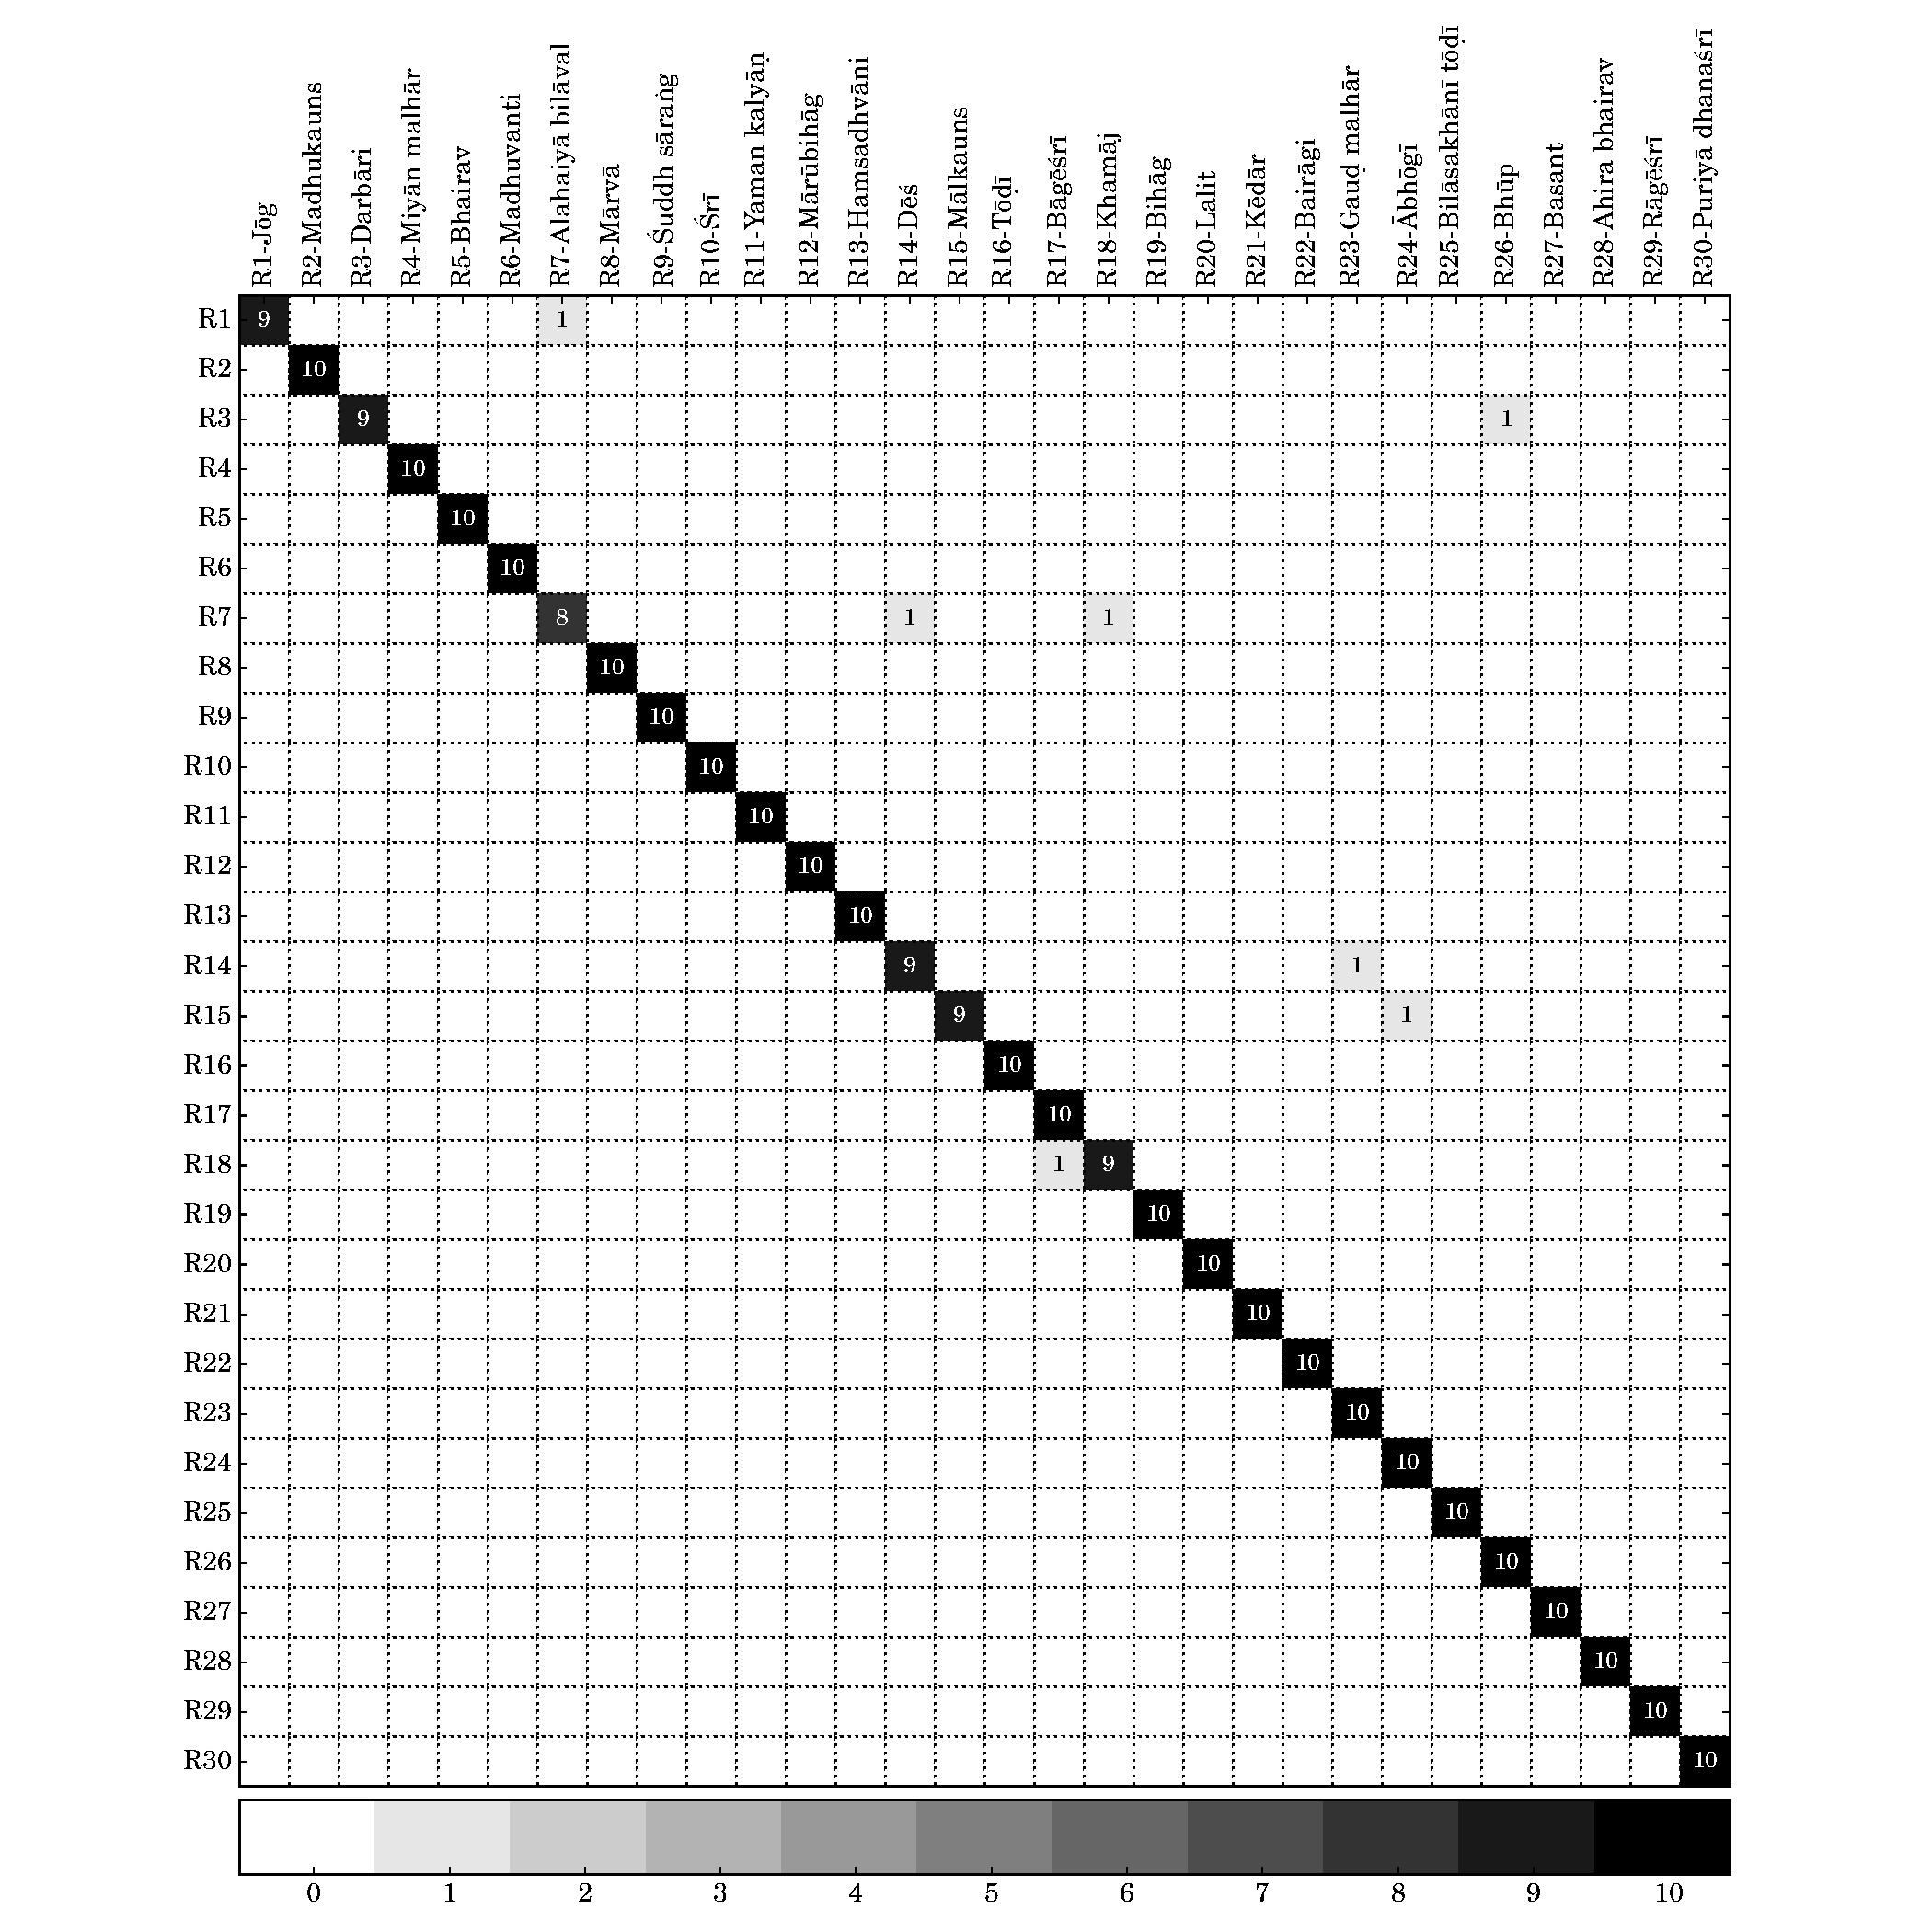
\includegraphics[width=\figSizeNinety]{ch07_ragaRecognition/figures/CM_tdms_hmd_var1.pdf}
	\end{center}
	\caption{Confusion matrix of the \gls{raga} predictions by \acrshort{ragarecTDMS} on \acrshort{rrds_hmd_big} dataset. The different shades of grey are mapped to different number of audio recordings.}
	\label{fig:confusion_matrix_hmd_tdms}
\end{figure}


